%%% Do not change from BEGIN to END
%%% BEGIN
\documentclass[a4paper,10pt]{article}

\usepackage[utf8]{inputenc}
\usepackage[T1]{fontenc}
\usepackage[danish,english]{babel}
\usepackage{graphicx}
\usepackage[a4paper,margin=2.7cm]{geometry}

\usepackage[math]{kurier}

\usepackage{amsmath}
\usepackage{amssymb}
\usepackage{amsfonts}
\usepackage{enumerate}

\usepackage{tikz}
\usetikzlibrary{arrows,decorations.pathmorphing,backgrounds,positioning,fit,matrix}


\setlength{\parindent}{0pt}
\setlength{\parskip}{2ex} 


\renewcommand{\vec}[1]{\ensuremath {\mathbf #1}}

%%% Settings for the Instructor
\newcommand{\courseid}{DM559/DM545}
\newcommand{\coursename}{Linear and Integer Programming}
\newcommand{\term}{Spring 2017}
\newcommand{\dept}{Department of Mathematics and Computer Science}
%%%%%%%%%%%%%%%%%%%%%%%%%%%%%%%%%%%%%%%%%%%%%%%%%%%%%%%%%%%%

\usepackage{fancyhdr}
\usepackage{lastpage}
\usepackage{listings}
\lstset{language=Python,
  basicstyle=\ttfamily\lst@ifdisplaystyle\footnotesize\fi,%\fontfamily{pzc}\selectfont,%
  stringstyle=\ttfamily,
  commentstyle=\ttfamily,
  showstringspaces=false,
  frame=lines, 
  breaklines=true, tabsize=2,
  extendedchars=true,inputencoding=utf8
}
%\lstavoidwhitepre


\pagestyle{fancy} 
\lhead{{\sc \courseid -- \term }} 
\chead{}
\rhead{CPR~nr.~\idnr}
\cfoot{Page \thepage\ of \pageref{LastPage}}

\fancypagestyle{plain}{
\lhead{\dept\\
University of Southern Denmark, Odense}
\chead{}
\rhead{\today\\
ID~\idnr}
\lfoot{}
\rfoot{}
%\renewcommand{\headrulewidth}{0pt}
}


\title{\begin{flushleft}
\vspace{-4ex}
\courseid~-- \coursename \\[0.2cm]
{\Large Answers to Obligatory Assignment 1.2, \term \\[3ex]
\hrule}
\end{flushleft}
}


\date{}

%%% END

%%% Settings for the Student
%%%%%%%%%%%%%%%%%%%%%%%%%%%%%%%%%%%%%%%%%%%%%%%%%%%%%%%%%%%%
%%%%%%%%%%%%%%%%%%%%%%%%%%%%%%%%%%%%%%%%%%%%%%%%%%%%%%%%%%%%
\author{Mikkel Pilegaard(mipil15) \& Mathias Holst Gundersen(mgund15)}
%%%%%%%%%%%%%%%%%%%%%%%%%%%%%%%%%%%%%%%%%%%%%%%%%%%%%%%%%%%%
%%%%%%%%%%%%%%%%%%%%%%%%%%%%%%%%%%%%%%%%%%%%%%%%%%%%%%%%%%%%

\begin{document}
\maketitle

%%%%%%%%%%%%%%%%%%%%%%%%%%%%%%%%%%%%%%%%%%%%%%%%%%%%%%%%%%%%
%%%%%%%%%%%%%%%%%%%%%%%%%%%%%%%%%%%%%%%%%%%%%%%%%%%%%%%%%%%%
\section*{Task 1}
%%%%%%%%%%%%%%%%%%%%%%%%%%%%%%%%%%%%%%%%%%%%%%%%%%%%%%%%%%%%
%%%%%%%%%%%%%%%%%%%%%%%%%%%%%%%%%%%%%%%%%%%%%%%%%%%%%%%%%%%%

The first code snippet is the model implementation of the DFJ formulation. This is followed up by 3 code snippets, which are used by the solver.

\begin{lstlisting}
def solve_tsp(points, subtours = []):
    points=list(points)
    V = range(len(points))
    E = [(i,j) for i in V for j in V if i<j]
    E = tuplelist(E)

    m = Model("TSP0")
    m.setParam(GRB.param.Presolve, 0)
    m.setParam(GRB.param.Method, 0)
    m.setParam(GRB.param.MIPGap,1e-7)

    ######### BEGIN: Write here your model for Task 1   

    # Decision Variables
    tmp = []
    
    roads = {}
    for (a,b) in E:
        road = m.addVar(lb=0, ub=1, vtype=GRB.BINARY, name="road"+str((a,b)))
        roads[(a,b)] = road
        tmp += [road * distance(points[a], points[b])]

    # Set the objective function
    m.setObjective( quicksum(tmp), GRB.MINIMIZE )
      
    # Constraint to make sure we have exactly 2 roads for each city
    for i in V:
        m.addConstr( quicksum( roads[(a,b)] for (a,b) in delta([i], V) ), GRB.EQUAL, 2, name="c1_"+str(i)+str((a,b)))
    
    # Constraint to remove subtours
    for i in subtours:
        if len(i) < 2:
            continue
        m.addConstr( quicksum( roads[(a,b)] for (a,b) in Edges(i)) <= len(i) - 1 )
    
    ######### END
    
    m.optimize()
    m.write("tsplp.lp")
    
    if m.status == GRB.status.OPTIMAL:
        print('The optimal objective is %g' % m.objVal)
        m.write("tsplp.sol") # write the solution
        return {(i,j) : roads[(i,j)].x for i,j in E}
    else:
        print "Something wrong in solve_tsplp"
        exit(0)

# Creating the subset of cities
sets = list(powerset(range(len(ran_points))))
# The first element of the list is the empty set and the last element is the full set, hence we remove them.
sets = sets[1:(len(sets)-1)]
solve_tsp(ran_points, sets) Don't solve
\end{lstlisting}

Creates a powerset from an iterable object, such as a tuple or a list.

\begin{lstlisting}
def powerset(iterable):
    "powerset([1,2,3]) --> () (1,) (2,) (3,) (1,2) (1,3) (2,3) (1,2,3)"
    s = list(iterable)
    return chain.from_iterable(combinations(s, r) for r in range(len(s)+1))
\end{lstlisting}

Creates a list of edges from the set of vertices given. Creates an edges from every city to every other city, but only 1 edge between the same cities.

\begin{lstlisting}
def Edges(vertices):
    """Takes a set of vertices and returns a set of edges from those vertices. 
    Also edges should be ordered by ij if i < j or ji if j < i"""
    # Every vertex is connected to each other, so therefore we can construct the edges like this
    E = [(i,j) for i in vertices for j in vertices if i<j]
    return E
\end{lstlisting}

Finds the edges in the cut v in the set of vertices V.

\begin{lstlisting}
def delta(v, V):
    """The set of edges in the cut (v, V\{v})"""
    E = [(i,j) for i in v for j in V if i<j]
    D = [(j,i) for i in v for j in V if j<i]
    return E+D
\end{lstlisting}


%%%%%%%%%%%%%%%%%%%%%%%%%%%%%%%%%%%%%%%%%%%%%%%%%%%%%%%%%%%%
\newpage
\section*{Task 2}
%%%%%%%%%%%%%%%%%%%%%%%%%%%%%%%%%%%%%%%%%%%%%%%%%%%%%%%%%%%%

When removing the integrality constraint and the subtour elimination constraint, the solution contains variables which are not all integers. When the resulting route has non-integer values, we do not have a complete tour, and this also means that the matrix cannot be TUM. \textbf{Han sagde noget i timen med at Andreas' svar ikke var 'nok', så måske der skal mere eller anden forklaring til?}

And since the subtour elimination constraint has been removed, if just 2 or more points are grouped up, we will expect a subtour.

%%%%%%%%%%%%%%%%%%%%%%%%%%%%%%%%%%%%%%%%%%%%%%%%%%%%%%%%%%%%
%%%%%%%%%%%%%%%%%%%%%%%%%%%%%%%%%%%%%%%%%%%%%%%%%%%%%%%%%%%%
\newpage
\section*{Task 3}
%%%%%%%%%%%%%%%%%%%%%%%%%%%%%%%%%%%%%%%%%%%%%%%%%%%%%%%%%%%%
%%%%%%%%%%%%%%%%%%%%%%%%%%%%%%%%%%%%%%%%%%%%%%%%%%%%%%%%%%%%
We solved the relaxed version of the TSP problem and received this result:

\begin{figure}[htb]
\begin{center}
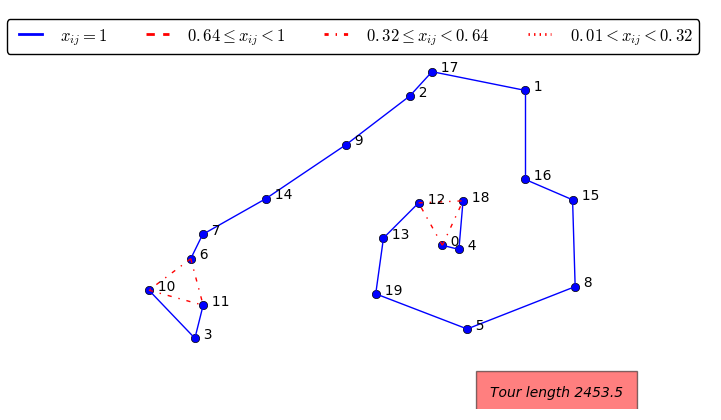
\includegraphics[scale=0.7]{task31.png}
\end{center}
\end{figure}

Then we visually inspect the solution, and choose the subtour [3,10,11], add it to the solvers parameters, solve the model, again and get this new result:

\begin{figure}[htb]
\begin{center}
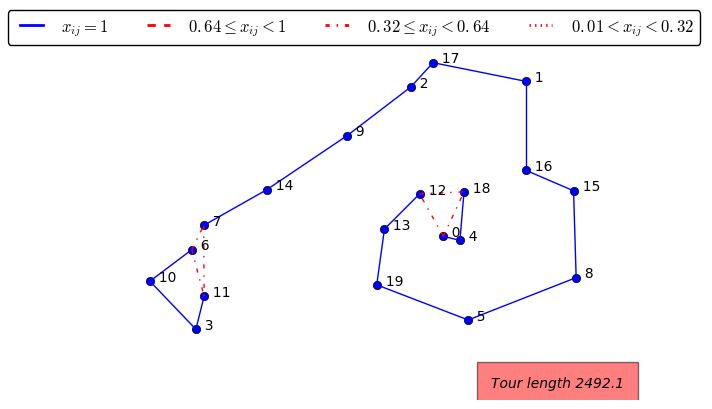
\includegraphics[scale=0.7]{task32.png}
\end{center}
\end{figure}

Then we inspect the result again, find the subtour [3,6,10,11] and add it to our list of subtour, and pass it to the solver, and solve again. This we continue until no more subtour can be found.

The final subtour list and the plotted result was:

\begin{lstlisting}
tsplp1 = solve_tsp0(ran_points, [(3,10,11),(3,6,10,11),(3,6,7,10,11),(0,4,18),(0,4,12,18),(3,6,7,10,11,14)])
plot_situation(ran_points, tsplp1)
\end{lstlisting}

\begin{figure}[htb]
\begin{center}
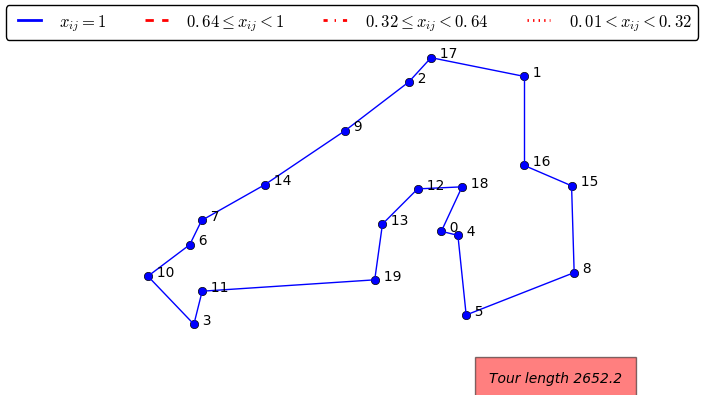
\includegraphics[scale=0.7]{task33.png}
\end{center}
\end{figure}

\textbf{"Show your last solution and comment on it."}

%%%%%%%%%%%%%%%%%%%%%%%%%%%%%%%%%%%%%%%%%%%%%%%%%%%%%%%%%%%%
%%%%%%%%%%%%%%%%%%%%%%%%%%%%%%%%%%%%%%%%%%%%%%%%%%%%%%%%%%%%
\newpage
\section*{Task 4}
%%%%%%%%%%%%%%%%%%%%%%%%%%%%%%%%%%%%%%%%%%%%%%%%%%%%%%%%%%%%
%%%%%%%%%%%%%%%%%%%%%%%%%%%%%%%%%%%%%%%%%%%%%%%%%%%%%%%%%%%%

When looking at the separation problem in the assignment, we can see that it is not a linear problem, since the variables $z_i$ and $z_j$ are multiplied together. We want to rewrite this to a linear problem, and we do so by observing that both variables are binary, and when multiplied together, they act as the logical condition AND. The AND condition can be rewritten as a linear condition. This is done for our SEP problem:

Objective function:
$$ \max \sum_{e=ij\in E':i < j} x^*_e y_e - \sum_{i \in V' \setminus \{k\}} z_i $$
Constraints:
$$ z_k = 1 $$
$$ y_{ij} \geq z_i + z_j - 1 \quad \forall ij \in E' $$
$$ y_{ij} \leq z_i,z_j \quad \forall ij \in E' $$
$$ y_{ij} \geq 0 \quad \forall ij \in E' $$
$$ z \in \mathbb{B}^n $$

%%%%%%%%%%%%%%%%%%%%%%%%%%%%%%%%%%%%%%%%%%%%%%%%%%%%%%%%%%%%
%%%%%%%%%%%%%%%%%%%%%%%%%%%%%%%%%%%%%%%%%%%%%%%%%%%%%%%%%%%%
\newpage
\section*{Task 5}
%%%%%%%%%%%%%%%%%%%%%%%%%%%%%%%%%%%%%%%%%%%%%%%%%%%%%%%%%%%%
%%%%%%%%%%%%%%%%%%%%%%%%%%%%%%%%%%%%%%%%%%%%%%%%%%%%%%%%%%%%

\textbf{Do we get the expected answer?}

\begin{lstlisting}
def solve_separation(points, x_star, k):
    points=list(points)
    V = range(len(points))
    Vprime = range(1,len(points))
    E = [(i,j) for i in V for j in V if i<j]
    Eprime = [(i,j) for i in Vprime for j in Vprime if i<j]
    E = tuplelist(E)
    Eprime = tuplelist(Eprime)

    m = Model("SEP")
    m.setParam(GRB.param.OutputFlag,0)
    
    ######### BEGIN: Write here your model for Task 4

    # Decision variables
    z_values = {}
    right_objective = []
    for i in Vprime:
        z_values[i] = m.addVar(lb = 0, ub = 1, vtype = GRB.INTEGER, name = "z_" + str(i))
        if i != k:
            right_objective += [z_values[i]]
    
    y_values = {}
    left_objective = []
    for (i, j) in Eprime:
        if i < j:
            y_values[(i, j)] = m.addVar(lb = 0, ub = 1, vtype = GRB.INTEGER, name = "y_" + str((i, j)))
            left_objective += [x_star[(i, j)] * y_values[(i, j)]]
    
    m.setObjective(quicksum(left_objective) - quicksum(right_objective), GRB.MAXIMIZE)
    
    # Add constraints
    
    m.addConstr(z_values[k] == 1)
    
    for (i, j) in Eprime:
        m.addConstr(y_values[(i, j)] >= z_values[i] + z_values[j] - 1)
        m.addConstr(y_values[(i, j)] <= z_values[i])
        m.addConstr(y_values[(i, j)] <= z_values[j])
            
    
    ######### END
    m.optimize()
    #m.write("sep.lp")
    
    if m.status == GRB.status.OPTIMAL:
        print('Separation problem solved for k=%d, solution value %g' % (k,m.objVal))
        #m.write("sep.sol") # write the solution    
        subtour = filter(lambda i: z_values[i].x>=0.99, z_values)
        return m.objVal, subtour
    else:
        print "Something wrong in solve_tsplp"
        exit(0)
\end{lstlisting}

%%%%%%%%%%%%%%%%%%%%%%%%%%%%%%%%%%%%%%%%%%%%%%%%%%%%%%%%%%%%
%%%%%%%%%%%%%%%%%%%%%%%%%%%%%%%%%%%%%%%%%%%%%%%%%%%%%%%%%%%%
\newpage
\section*{Task 6}
%%%%%%%%%%%%%%%%%%%%%%%%%%%%%%%%%%%%%%%%%%%%%%%%%%%%%%%%%%%%
%%%%%%%%%%%%%%%%%%%%%%%%%%%%%%%%%%%%%%%%%%%%%%%%%%%%%%%%%%%%

If we run our random seed with continuous variables, we find a solution. If we run the dantzig42 with continuous variables, we do not get a solution, but if we use integer variables, we get a solution. 

\begin{lstlisting}
def cutting_plane_alg(points):
    Vprime = range(1,len(points))
    subtours = []
    found = True
    while found:
        lpsol = solve_tsp0(points,subtours)
        # plot_situation(points, lpsol)
        found = False
        tmp_subtours = []
        best_val = float('-inf')
        for k in Vprime:
            value, subtour = solve_separation(points,lpsol,k)
            best_val = value if value > best_val else best_val
            ######### BEGIN: write here the condition. Include a tollerance
            if value > 0.49: 
            ######### END
                found = True
                tmp_subtours += [subtour]
        subtours += tmp_subtours
        print '*'*60
        print "********** Subtours found: ",tmp_subtours," with best value : ",best_val
        print '*'*60
    plot_situation(points, lpsol)
    
cutting_plane_alg(dantzig42)
\end{lstlisting}

\textbf{Mangler at indsætte plot af sidste løsning, samt hvor mange iterationer det tog.}

%%%%%%%%%%%%%%%%%%%%%%%%%%%%%%%%%%%%%%%%%%%%%%%%%%%%%%%%%%%%
%%%%%%%%%%%%%%%%%%%%%%%%%%%%%%%%%%%%%%%%%%%%%%%%%%%%%%%%%%%%
\newpage
\section*{Task 9}
%%%%%%%%%%%%%%%%%%%%%%%%%%%%%%%%%%%%%%%%%%%%%%%%%%%%%%%%%%%%
%%%%%%%%%%%%%%%%%%%%%%%%%%%%%%%%%%%%%%%%%%%%%%%%%%%%%%%%%%%%

\textbf{Tour length:} 2652,2

\end{document}
          



